\documentclass[9pt, aspectratio=169]{beamer}
\usepackage{FiraSans}
\usetheme{metropolis}
\usepackage[utf8]{inputenc}
\usepackage{amsmath}
\usepackage{amsfonts}
\usepackage{amssymb}
\usepackage{multicol}
\usepackage{tikz}
\usepackage{xcolor}
\usepackage[T1]{fontenc} 
\usepackage[skins]{tcolorbox}
\author{Nicola Roman\`o - nicola.romano@ed.ac.uk}
\title{Lecture 2 - Geometric image transformations}
\setlength{\fboxsep}{0pt}
\setbeamertemplate{caption}{\raggedright\insertcaption\par}
\setbeamertemplate {footline}{\begin{scriptsize}\hfill\insertframenumber ~of \inserttotalframenumber\kern1em\vskip5pt\end{scriptsize}}

\definecolor{darkgreen}{rgb}{0, 0.5, 0}

%\setbeamercovered{transparent} 
%\setbeamertemplate{navigation symbols}{} 

\titlegraphic{\centering 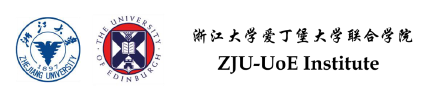
\includegraphics[scale=.5]{instituteLogo.png}}
\date{}

\AtBeginSection[]
{
  \begin{frame}<beamer>
    {Outline}
    \huge{\tableofcontents[currentsection, currentsubsection]}
  \end{frame}
}

\AtBeginSubsection[]
    {
    \begin{frame}<beamer>
        {Outline}
        \huge{\tableofcontents[currentsection, currentsubsection]}
        \end{frame}        
    }

\begin{document}

\newtcolorbox{codebox}{enhanced,
    top=2pt,
    left=2pt,
    right=2pt,
    bottom=2pt,
    boxrule=0pt,
    leftrule=5pt,
    sharp corners,
    colback=gray!20,
    colframe=blue!60!black}

\begin{frame}
    \titlepage
\end{frame}

\section{A brief recap}

\begin{frame}
    {Python tools for image processing}
    \centering
    Last time we learnt how to open and display images using Python.

    \vspace{3em}

    \begin{columns}
        \begin{column}{0.3\textwidth}
            
\includegraphics[width=0.8\textwidth]{matplotlib_logo.png}
            General plotting library
        \end{column}
        \begin{column}{0.3\textwidth}
            
\includegraphics[width=0.8\textwidth]{skimage_logo.png}
            Specific functions for image manipulation
        \end{column}
        \begin{column}{0.3\textwidth}
            
\includegraphics[width=0.8\textwidth]{numpylogo.png}
            Library for matrix operations
        \end{column}
    \end{columns}
\end{frame}

\begin{frame}
    {Reading images as Numpy arrays}
    \begin{columns}
        \begin{column}{0.5\textwidth}
            \begin{center}
                
\includegraphics[width=0.5\textwidth]{matplotlib_logo.png}
            \end{center}
            \begin{codebox}
                \texttt{import matplotlib.pyplot as plt\\
                    \texttt{img = plt.imread(}"cells.jpg")\\
                    plt.imshow(\texttt{img)\\
                        plt.show(})
                }
            \end{codebox}
        \end{column}
        \begin{column}{0.5\textwidth}
            \begin{center}
                
\includegraphics[width=0.5\textwidth]{skimage_logo.png}
            \end{center}
            \begin{codebox}
                \texttt{from skimage import io\\
                    \texttt{img = io.imread(}"cells.jpg")\\
                    io.imshow(\texttt{img)\\
                        io.show(})
                }
            \end{codebox}
        \end{column}
    \end{columns}
\end{frame}

\begin{frame}
    {Colour mapping}
    \begin{columns}
        \begin{column}{0.6\textwidth}
            \begin{codebox}
                \texttt{fig, ax = plt.subplots(ncols=2, nrows=2)\\
                    ax[0, 0].imshow(img, cmap="gray")\\
                    ax[0, 1].imshow(img, cmap="viridis")\\
                    ax[1, 0].imshow(img, cmap="Greens")\\
                    ax[1, 1].imshow(img, cmap="PuBu")\\
                    plt.show()}
            \end{codebox}
        \end{column}
        \begin{column}{0.4\textwidth}
            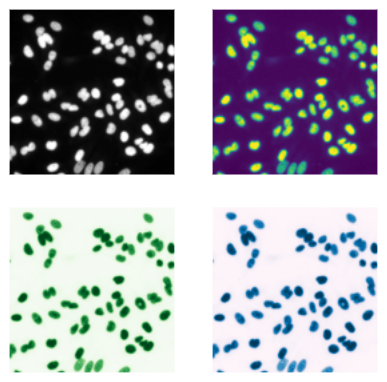
\includegraphics[width=\textwidth]{nuclei_cmapped.png}
        \end{column}
    \end{columns}
    \centering

    Check out the Matplotlib website for a list of colourmaps! \url{https://matplotlib.org/stable/tutorials/colors/colormaps.html}

\end{frame}

\begin{frame}
    {Learning objectives}
    \begin{columns}
        \begin{column}{0.8\textwidth}
            \begin{itemize}
                \item Describe use cases for geometric transformations of images
                \item Use Python to crop images (in 2 or more dimensions)
                \item Explain the theory of affine transformations
                \item Implement basic transformations in Python (translation, scaling, rotation)
            \end{itemize}
        \end{column}
        \begin{column}{0.2\textwidth}
            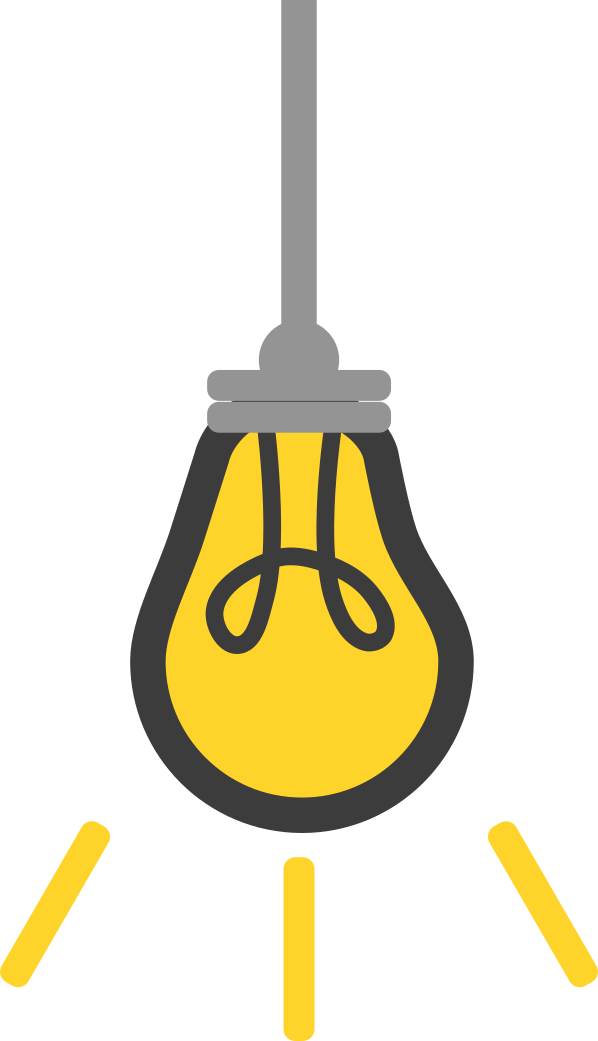
\includegraphics[angle=-30, origin=tr, width=1.5\textwidth]{lightbulb.png}
        \end{column}
    \end{columns}
\end{frame}

\section{Geometric image transformations}

\begin{frame}
    {Geometric image transformations}
    \textbf{Geometric image transformations} are operations that change the image geometry without altering its pixel values (mostly\dots).

    Examples are cropping, translating, scaling rotating an image.\\
    \pause
    Example use cases:

    \begin{itemize}
        \item Analysing only part of an image (cropping)
        \item Making sure all input images for a pipeline are the same size (scaling, cropping)
        \item Aligning multiple images (e.g. in video stabilization) (rotating, translating)
        \item \dots
    \end{itemize}
    \begin{center}
        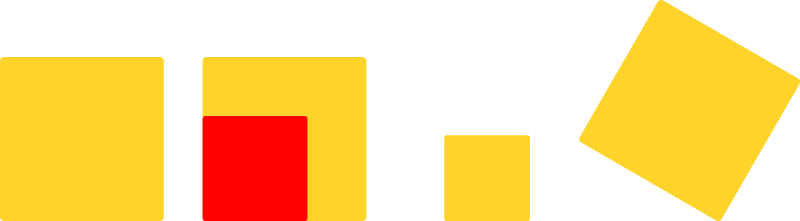
\includegraphics[width=0.4\textwidth]{basic_manipulation.png}
    \end{center}
\end{frame}

\subsection{Cropping}

\begin {frame}
{Cropping}
Cropping is as easy as subsetting the image matrix.


\begin{columns}
    \begin{column}{0.6\textwidth}
        \begin{codebox}
            {\texttt{\# img contains a 512 x 512 image\\
                    \# Take the top-left 100 x 100 pixels\\
                    img1 = img[0:100, 0:100] \# shape (100, 100)\\
                    \onslide<2->
                    {\\
                        \# A 100 pixel wide strip on the left\dots\\
                        img2 = img[:, 0:100] \# shape (512, 100)\\
                        \# \dots or on the right!\\
                        img3 = img[:, -100:] \# shape (512, 100)
                    }
                }
            }
        \end{codebox}
    \end{column}
    \begin{column}{0.4\textwidth}
        \only<1>{
            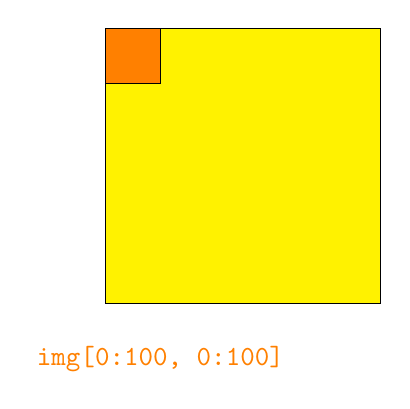
\begin{tikzpicture}[scale=0.7]
                \draw [fill=yellow]  (0,0) rectangle (5,5);
                \draw [fill=orange]  (0, 4) rectangle (1,5);
                \draw node at (1, -1) {\color{orange}\texttt{img[0:100, 0:100]}};
            \end{tikzpicture}
        }
        \only<2>{
            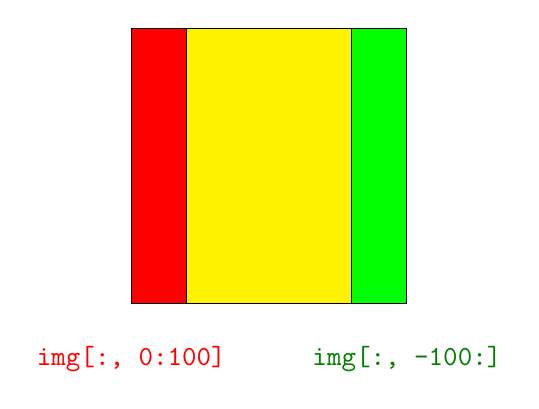
\begin{tikzpicture}[scale=0.7]
                \draw [fill=yellow]  (0,0) -- (0,5) -- (5,5) -- (5,0) -- cycle;
                \draw [fill=red]  (0,0) -- (0,5) -- (1,5) -- (1,0) -- cycle;
                \draw [fill=green]  (4,0) -- (5,0) -- (5,5) -- (4,5) -- cycle;
                \draw node at (0, -1) {\texttt{\color{red}img[:, 0:100]}};
                \draw node at (5, -1) {\texttt{\color{darkgreen}img[:, -100:]}};
            \end{tikzpicture}
        }
    \end{column}
\end{columns}
\end{frame}

\begin{frame}
    {Cropping in more than two dimensions}
    Since images are just tensors, we can crop them in any dimension.
    \begin{columns}
        \begin{column}{0.6\textwidth}
            \begin{codebox}
                {
                    \texttt{
                        \# img is a 512 x 512 RGB image\\
                        \# img.shape is (3, 512, 512)\\
                        \# Extract the green channel\\
                        img\_green = img[1] \# Shape (512, 512)\\
                        \onslide<2->{\\
                            \# video is a 512 x 512 video of 300 frames\\
                            \# video.shape is (300, 512, 512)\\
                            \# Take the first 50 frames\\
                            video\_crop = video[0:50]
                        }
                    }
                }
            \end{codebox}
        \end{column}
        \begin{column}{0.4\textwidth}
            \only<1>{
                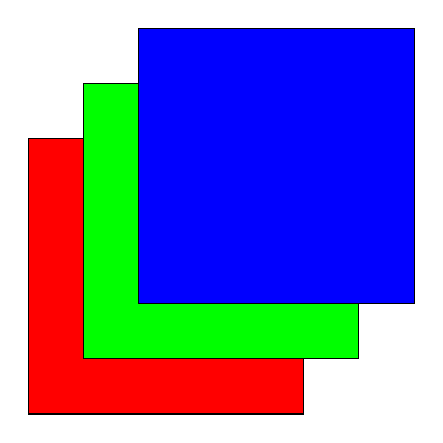
\begin{tikzpicture}[scale=0.7]
                    \draw [fill=red]  (0,0) rectangle (5,5);
                    \draw [fill=green]  (1,1) rectangle (6,6);
                    \draw [fill=blue]  (2,2) rectangle (7,7);
                \end{tikzpicture}
            }
            \only<2>{
                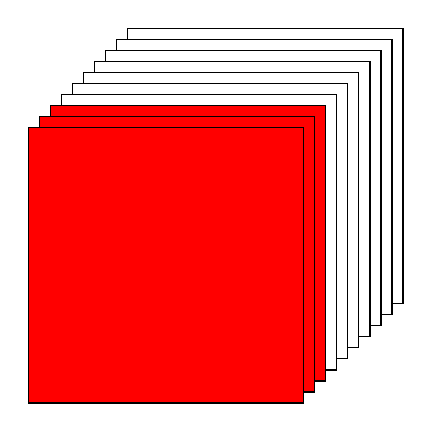
\begin{tikzpicture}[scale=0.7]
                    \foreach \i in {2,1.8,...,0.6}
                        {
                            \draw [fill=white] (\i, \i) rectangle (\i+5, \i+5);
                        }
                    \foreach \i in {0.6,0.4,...,0}
                        {
                            \draw [fill=red] (\i, \i) rectangle (\i+5, \i+5);
                        }
                \end{tikzpicture}
            }
        \end{column}
    \end{columns}
\end{frame}

\begin{frame}
    {Question time}
    \begin{columns}
        \begin{column}{0.7\textwidth}
            We have a 100 frames video of a 512 x 512 z-stack with 60 planes loaded in \texttt{zstack}.\\
            \texttt{zstack.shape} is \texttt{(100, 60, 512, 512)}\\
            \vspace*{2em}
            \centering
            \textbf{What does this code give you?}
            \vspace{2em}
            \begin{codebox}
                \texttt{result = stack[50:70, :, 100:300]}
            \end{codebox}
        \end{column}
        \begin{column}{0.3\textwidth}
            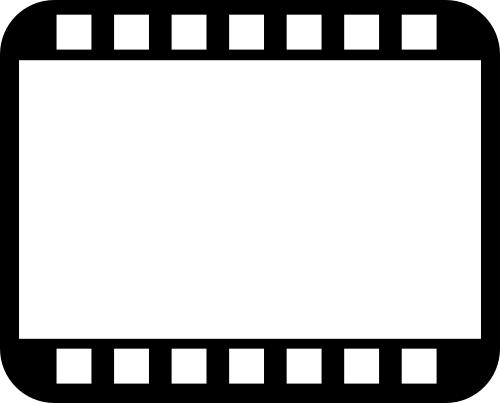
\includegraphics[width=.7\textwidth]{video.png}
        \end{column}
    \end{columns}
\end{frame}

\begin{frame}
    {Affine transformations}
    In Euclidean geometry, an affine transformation is a geometric transformation that preserves lines and parallelism but not necessarily distances and angles. [Wikipedia]
    \vspace{2em}

    \begin{columns}
        \begin{column}{0.5\textwidth}{
                \centering
                \begin{tikzpicture}
                    \draw [thin, ->] (1,2) -- (3,1);
                    \fill[red] (1, 2) circle (2pt) node at (1, 2.3) {$P$};
                    \fill[red] (3.1, 1) circle (2pt) node at (3.3, 1) {$P'$};
                \end{tikzpicture}

                We want to transform $P~(x;y)$ into $P'~(x';y')$.

                $$P': \begin{cases}x' = f(x,y)\\y' = g(x,y)\end{cases}$$

                \begin{center}
                    Where $f$ and $g$ are linear functions.
                \end{center}
            }
        \end{column}
        \pause
        \begin{column}{0.5\textwidth}
            {We can generalise this to an image, by applying the transformation to every pixel.
                \begin{center}
                    {
                        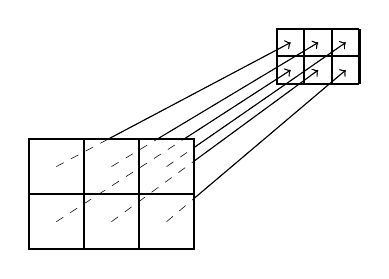
\begin{tikzpicture}[scale=0.7]
                            \foreach \x in {0.5,1.5,2.5}
                                {
                                    \draw [thin, ->] (\x,1.5) -- (\x/2+4.5,3.75);
                                    \draw [thin, ->] (\x,0.5) -- (\x/2+4.5,3.25);
                                }
                            \draw [thick, fill=white] (0,0) rectangle (3,2);
                            \draw [thick] (0,0) grid (3,2);
                            \draw [thick, step=0.5] (4.49,2.99) grid (6,4);

                            \foreach \x in {0.5,1.5,2.5}
                                {
                                    \draw [very thin, dashed, ->] (\x,0.5) -- (\x/2+4.5,3.25);
                                    \draw [very thin, dashed, ->] (\x,1.5) -- (\x/2+4.5,3.75);
                                }

                            % \draw [thin, dotted] (0,2) -- (4.5,4);
                            % \draw [thin, dotted] (3,2) -- (6,4);
                            % \draw [thin, dotted] (3,0) -- (6,3);
                        \end{tikzpicture}
                    }
                \end{center}
            }
        \end{column}
    \end{columns}
\end{frame}

\subsection{Scaling}

\begin{frame}
    {Scaling}

    \begin{columns}
        \begin{column}{0.4\textwidth}
            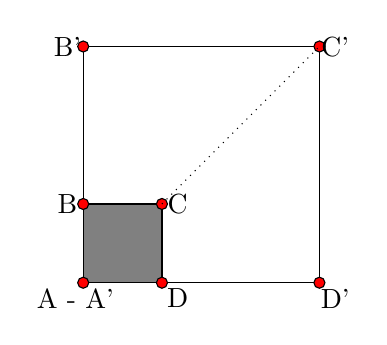
\begin{tikzpicture}
                \draw[thin, fill=white] (0,0) rectangle (3,3);
                \draw[thin, fill=gray] (0,0) rectangle (1,1);
                \draw[fill=red] (0, 0) circle (2pt) node at  (-.1, -.2) {A - A'};
                \draw[fill=red] (0, 1) circle (2pt) node at  (-.2, 1) {B};
                \draw[fill=red] (1, 1) circle (2pt) node at  (1.2, 1) {C};
                \draw[fill=red] (1, 0) circle (2pt) node at  (1.2, -0.2) {D};
                \draw[fill=red] (0, 3) circle (2pt) node at  (-.2, 3) {B'};
                \draw[fill=red] (3, 3) circle (2pt) node at  (3.2, 3) {C'};
                \draw[fill=red] (3, 0) circle (2pt) node at  (3.2, -0.2) {D'};
                \draw[dotted] (1,1) -- (3,3);
            \end{tikzpicture}
        \end{column}
        \begin{column}{0.6\textwidth}
            Scaling transforms the coordinates as:

            $$\begin{cases}x' = s_x * x\\y' = s_y * y\end{cases}$$
            \pause
            We can write this in matrix form\textsuperscript{*}:

            $$\begin{bmatrix}x'\\y'\end{bmatrix} = \color{red}\begin{bmatrix}s_x&0\\0&s_y\end{bmatrix}\color{black}\begin{bmatrix}x\\y\end{bmatrix}$$

            \begin{center}
                This is called the scaling \color{red}\textbf{transformation matrix}.\\
                \color{black}
            \end{center}

            \footnotesize
            \textsuperscript{*} Don't remember how matrix multiplication works? Check out \href{https://en.wikipedia.org/wiki/Matrix_multiplication}{\underline{Wikipedia}}!
        \end{column}
    \end{columns}
\end{frame}

\begin{frame}
    {Scaling}
    \centering
    
\includegraphics[width=.5\textwidth]{scaling.png}\\
    Two problems:\\
    When \textbf{upscaling} we need to generate new information.
    \\
    When \textbf{downscaling} we need to decide "how to lose" information.

    \textbf{Interpolation} is the solution!
\end{frame}

\begin{frame}
    {Nearest-neighbour interpolation}
    The simplest way to resize an image is to use nearest-neighbour interpolation. Each pixel of the scaled image will have the colour of the nearest pixel in the original image.\\

    In this "1D" example, we resize a 1x2 image to 1x6

    \centering
    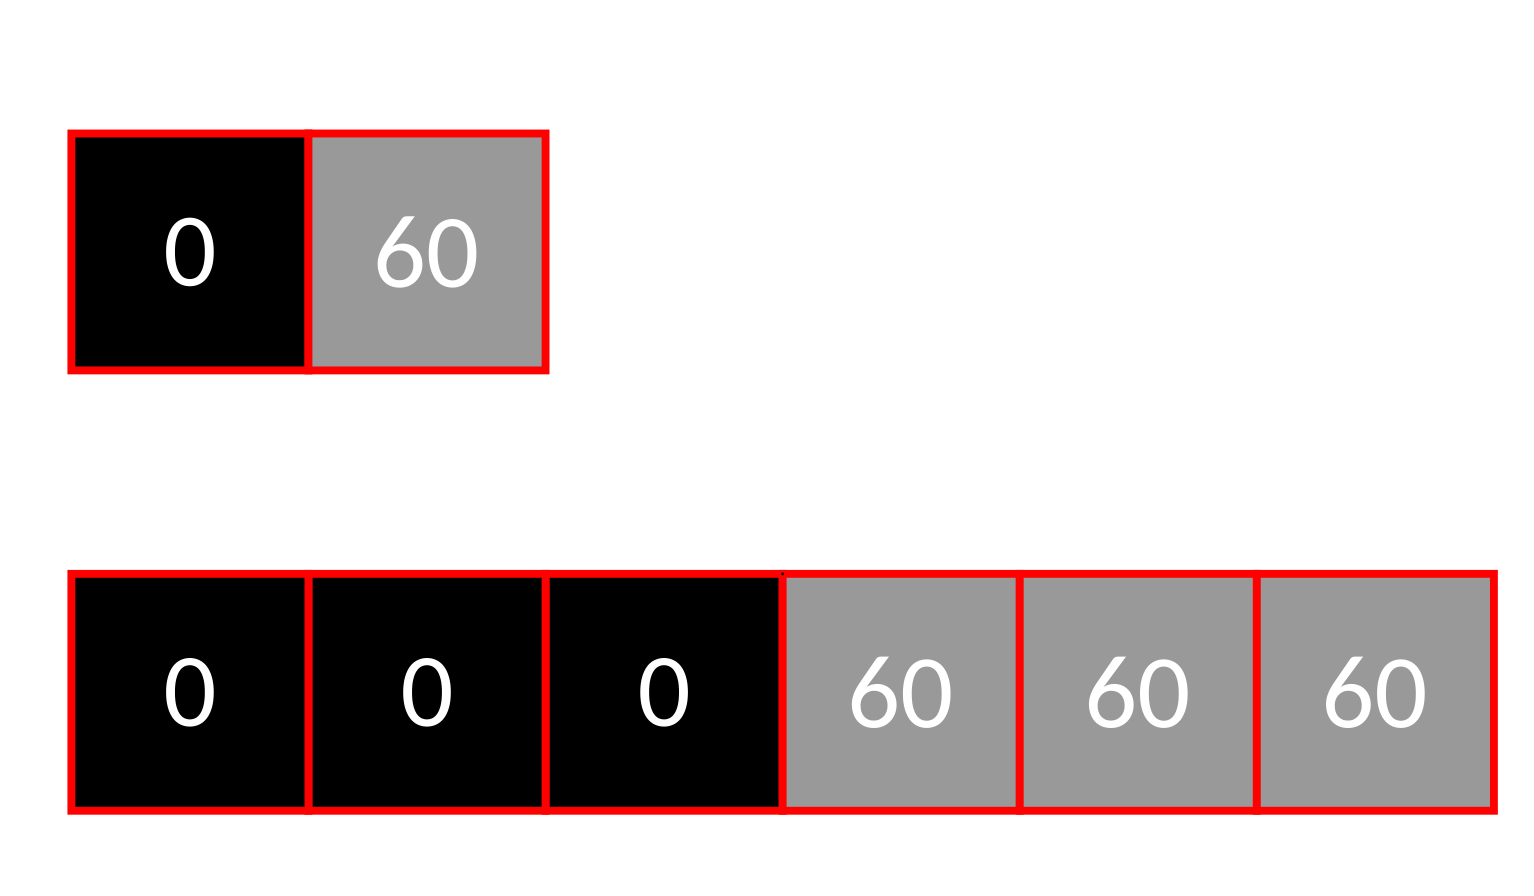
\includegraphics[width = 0.4\textwidth]{1D_NN_interpolation.png}
\end{frame}

\begin{frame}
    {Nearest-neighbour interpolation}
    \begin{figure}
        \centering
        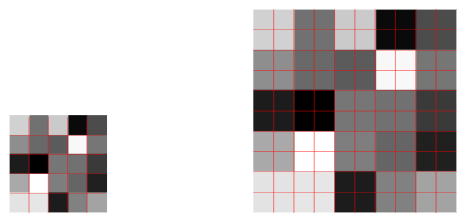
\includegraphics[width=.65\textwidth]{upscaling_no_interpolation.png}
        \caption{Upscaling of a 5x5 image by a factor of 2, to get a 10x10 image, with nearest neighbour interpolation}
    \end{figure}
    \pause
    \begin{codebox}
        \texttt{from skimage.transform import rescale\\
            \texttt{img\_scaled = rescale(}\texttt{img, 2, }order=0)}
    \end{codebox}
\end{frame}

\begin{frame}
    {Scaling with interpolation}
    Better ways to scale an image involve changing the pixel values of the rescaled image based on their neighbourhood.\\
    For example we could use linear interpolation
    \centering
    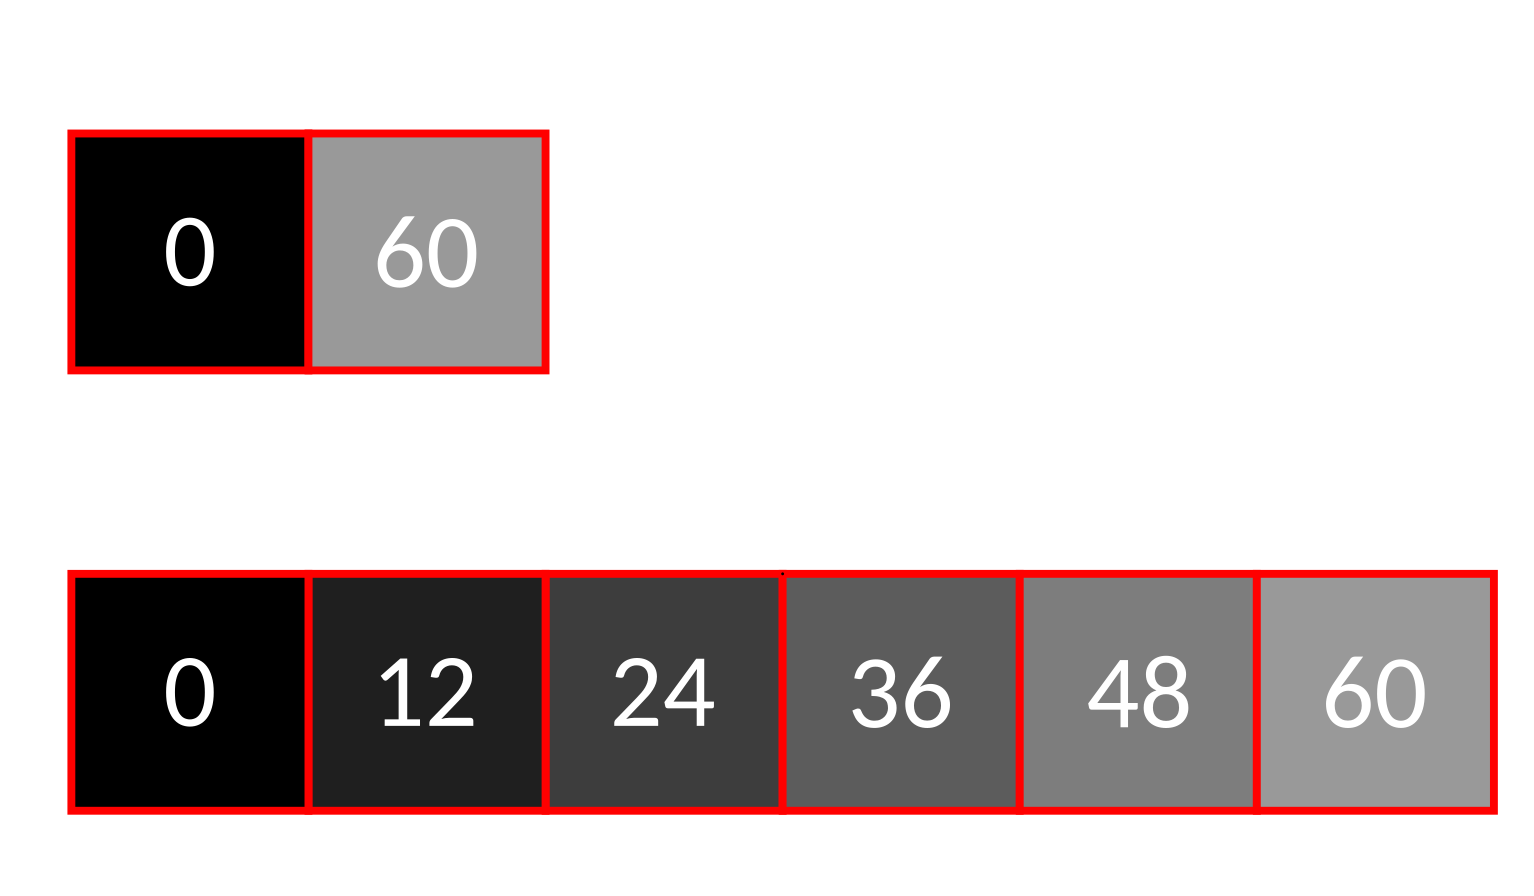
\includegraphics[width=0.65\textwidth]{1D_lin_interpolation.png}
\end{frame}

\begin{frame}
    {Linear interpolation}
    The same applies in 2D, although we need to take into accounts the values of both horizontal and vertical neighbours (\textbf{bilinear interpolation}).
    \begin{figure}
        \centering
        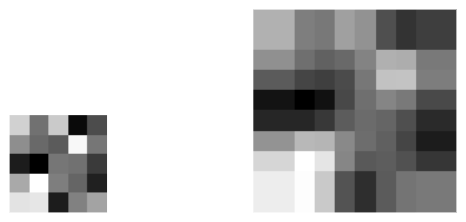
\includegraphics[width=.65\textwidth]{upscaling_lin_interpolation.png}
        \caption{Upscaling of a 5x5 image by a factor of 2, to get a 10x10 image, with bi-linear interpolation}
    \end{figure}

    \begin{codebox}
        \texttt{from skimage.transform import rescale\\
            \texttt{img\_scaled = rescale(}\texttt{img, 2, }order=1)}
    \end{codebox}
\end{frame}

\begin{frame}
    {Nearest neighbour vs linear interpolation}
    \begin{figure}

        \centering
        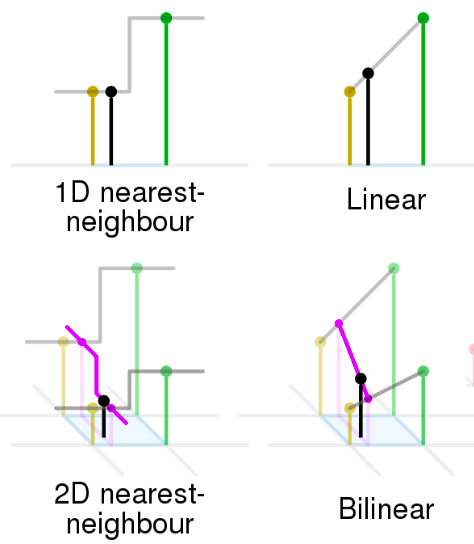
\includegraphics[width=0.4\textwidth]{interpolation schematics.png}
        \caption{Comparison of nearest neighbour and linear interpolation - Source: \href{https://en.wikipedia.org/wiki/Nearest-neighbor_interpolation}{Wikipedia}}
    \end{figure}
\end{frame}

\begin{frame}
    {Higher orders of interpolation}
    We can use higher orders of interpolation to produce smoother results. \\
    \begin{figure}

        \centering
        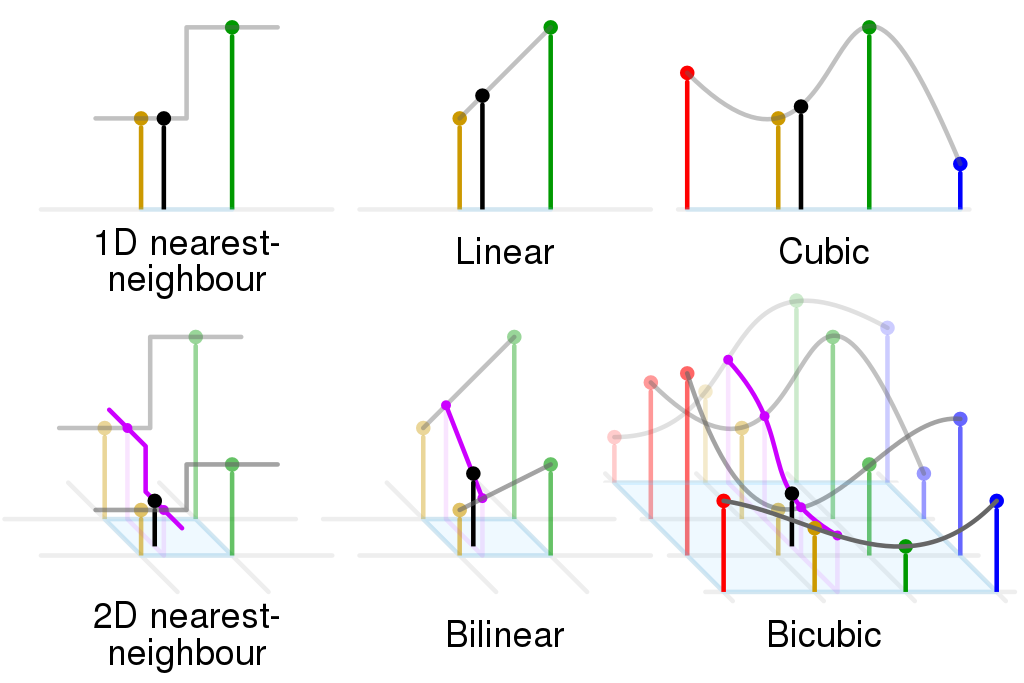
\includegraphics[width=0.55\textwidth]{interpolations.png}
        \caption{Comparison of nearest neighbour and linear interpolation - Source: \href{https://en.wikipedia.org/wiki/Nearest-neighbor_interpolation}{Wikipedia}}
    \end{figure}

    Scikit Image supports values from 0 to 5 in the \texttt{order} parameter of the \texttt{rescale} function. 0 is nearest neighbour, 1 is bi-linear, 2 is bi-quadratic and so on.
\end{frame}

\begin{frame}
    {Scaling to a target size}
    To scale to a target size, rather than by a specific factor, we can use \texttt{resize} instead of \texttt{rescale}.

    \begin{codebox}
        \texttt{import matplotlib.pyplot as plt\\
            from skimage.transform import resize, rescale\\
            \\
            \texttt{img = plt.imread(}"cells.jpg")\\
            \texttt{img\_scaled1 = rescale(}img, 2)\\
            img\_scaled2 = resize(img, (150, 150))
        }
    \end{codebox}
\end{frame}

\begin{frame}
    {Local mean downscaling}
    Another simple solution for downscaling is calculating the local mean of each pixel
    \centering
    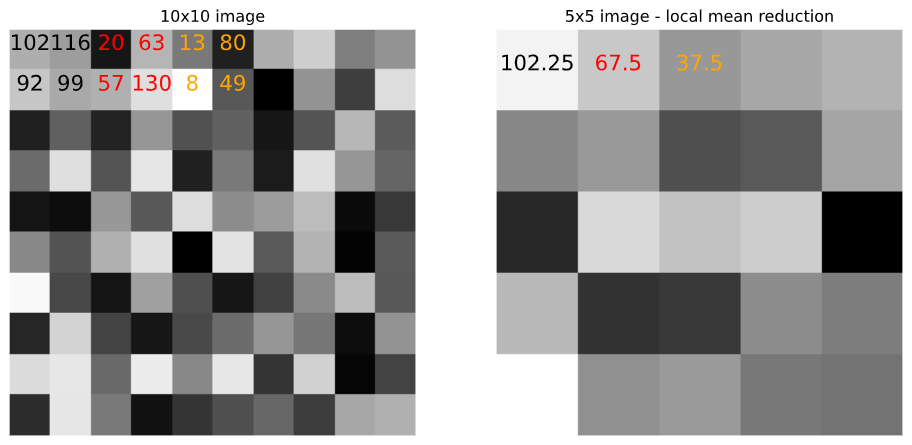
\includegraphics[width=.65\textwidth]{downscale.png}
    \pause
    \begin{codebox}
        \texttt{from skimage.transform import downscale\_local\_mean\\
            img\_small = downscale\_local\_mean(img, (2,2))}
    \end{codebox}

    Image needs to be padded if the size is not a multiple of the downscaling factor.\\
    This method is fast but not good at keeping fine details.
\end{frame}

\begin{frame}
    {Scaling summary}
    $$\begin{bmatrix}x'\\y'\end{bmatrix} = \begin{bmatrix}s_x&0\\0&s_y\end{bmatrix}\begin{bmatrix}x\\y\end{bmatrix}$$

    \texttt{skimage.transform.rescale} $\rightarrow$ scales an image by a specific factor (>1 upscaling; <1 downscaling.). Can specify a different scaling factor for each dimension of the image.
    \vspace{2em}

    \texttt{skimage.transform.resize} $\rightarrow$ scales an image to a target size.
    \vspace{2em}

    \texttt{skimage.transform.downscale\_local\_mean} $\rightarrow$ downscales the image by a specific factor (>1), using the local mean of each pixel.
\end{frame}

\subsection{Rotations}

\begin{frame}
    {Rotating a point around the origin}
    \centering
    We want to rotate a point $P (x,y)$ around the origin by an angle $\theta$ to get $P' (x',y')$.\\
    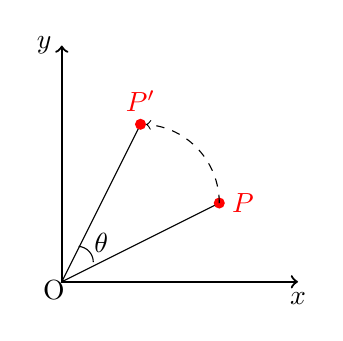
\begin{tikzpicture}
        \draw [<->,thick] (0,3) node (yaxis) [left] {$y$}
        |- (3,0) node (xaxis) [below] {$x$};
        \draw [thin] (1,2) -- (0,0) -- (2,1);
        \fill[red] (1, 2) circle (2pt) node at (1, 2.3) {$P'$};
        \fill[red] (2, 1) circle (2pt) node at (2.3, 1) {$P$};
        \draw [->, dashed] (2,1) arc (0:86:1);
        \draw (.4,.25) arc (0:86:.2) node at (.5, .5) {$\theta$};
        \node at (-.1, -.1) {O};
    \end{tikzpicture}
\end{frame}

\begin{frame}
    {Rotating a point around the origin}
    \center
    {
        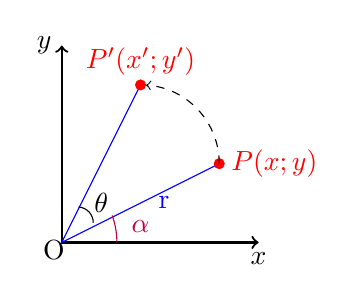
\begin{tikzpicture}
            % Axes
            \draw [<->,thick] (0,2.5) node (yaxis) [left] {$y$}
            |- (2.5,0) node (xaxis) [below] {$x$};
            \draw [thin, blue] (1,2) -- (0,0) -- (2,1);
            % Points
            \fill[red] (1, 2) circle (2pt) node at (1, 2.3) {$P' (x'; y')$};
            \fill[red] (2, 1) circle (2pt) node at (2.7, 1) {$P (x; y)$};
            % Rotation arrow
            \draw [->, dashed] (2,1) arc (0:86:1);
            % Angle theta
            \draw (.4,.25) arc (0:86:.2) node at (.5, .5) {$\theta$};
            % Angle alpha
            \draw [purple] (.7,0) arc (0:20:1) node at (1, .2) {$\alpha$};
            % Origin
            \node at (-.1, -.1) {O};
            % Radius
            \node [blue] at (1.3, .5) {r};
        \end{tikzpicture}
    }

    $$P: \begin{cases}x = r~\text{cos}(\alpha)\\y = r~\text{sin}(\alpha)\end{cases}
        P': \begin{cases}x' = r~\text{cos}(\alpha+\theta)\onslide<2->{= r~\text{cos}(\alpha)\text{cos}(\theta)-r~\text{sin}(\alpha)\text{sin}(\theta)}\\y' = r~\text{sin}(\alpha+\theta)\onslide<2->{= r~\text{sin}(\alpha)\text{cos}(\theta)+r~\text{sin}(\theta)\text{cos}(\alpha)}\end{cases}$$

    \pause
    \footnotesize
    Why? \href{https://en.wikipedia.org/wiki/List\_of\_trigonometric\_identities\#Angle\_sum\_and\_difference\_identities}{\underline{Wikipedia to the rescue!}}\\
    \pause
    \normalsize
    Thus:
    \begin{columns}
        \begin{column}{0.5\textwidth}
            $$P': \begin{cases}x' = x~\text{cos}(\theta)-y~\text{sin}(\theta)\\y' = y~\text{cos}(\theta)+x~{sin}(\theta)\end{cases}$$
        \end{column}
        \pause
        \begin{column}{0.5\textwidth}
            $$\begin{bmatrix}x'\\y'\end{bmatrix} = \color{red}\begin{bmatrix}\text{cos}\theta&-\text{sin}\theta\\\text{sin}\theta&\text{cos}\theta\end{bmatrix}\color{black}\begin{bmatrix}x\\y\end{bmatrix}$$
            \centering
            \color{red}Rotation transformation matrix
        \end{column}
    \end{columns}
\end{frame}

\begin{frame}
    {Rotating in Scikit Image}
    To rotate an image we will:
    \begin{itemize}
        \item Offset our image so that it is centered on the origin
        \item Generate a rotation matrix
        \item Multiply the coordinates of each pixel by the rotation matrix
        \item Shift back the image to its original position
    \end{itemize}
    \pause
    Luckily, Scikit Image has a function for that, \texttt{skimage.transform.rotate}.

    \begin{columns}
        \begin{column}{0.5\textwidth}
            \begin{codebox}
                \texttt{import matplotlib.pyplot as plt\\
                    from skimage.transform import rotate\\
                    \\
                    img = plt.imread("cells.jpg")\\
                    img\_rotated = rotate(img, 20)\\
                    \\
                    plt.imshow(img\_rotated, cmap="gray")\\
                    plt.show()}
            \end{codebox}
        \end{column}
        \begin{column}{0.5\textwidth}
            \begin{figure}
                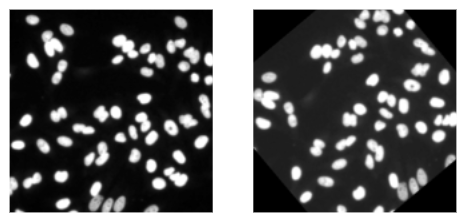
\includegraphics[width=\textwidth]{rotate_image.png}
                \caption{Note: we lost part of the image and we "gained" black pixels around it.}
            \end{figure}
        \end{column}
    \end{columns}
\end{frame}

\subsection{Translation}

\begin{frame}
    {Translation}
    To translate we offset the points by $(t_x, t_y)$: $\begin{cases}x' = x + t_x\\y' = y + t_y\end{cases}$

    The transformation matrix is different from the ones we saw for before:

    $\begin{bmatrix}x'\\y'\end{bmatrix} = \begin{bmatrix}x\\y\end{bmatrix} + \begin{bmatrix}t_x\\t_y\end{bmatrix}$

    \pause
    We can generate a transformation matrix using \texttt{SimilarityTransform} and apply it using \texttt{warp}.

    \begin{columns}
        \begin{column}{0.7\textwidth}
            \begin{codebox}
                \texttt{from skimage.transform import SimilarityTransform, warp\\
                    \# Create a 10x10 white image\\
                    img = np.ones(shape=(10, 10))\\
                    \# Make the central pixels black\\
                    img[5:7, 5:7] = 0\\
                    \\
                    m = SimilarityTransform(translate = (2, 5))\\
                    img\_translated = warp(img, m)
                }
            \end{codebox}
        \end{column}
        \pause
        \begin{column}{0.3\textwidth}
            
\includegraphics[width=.6\textwidth]{translation.png}
        \end{column}
    \end{columns}
\end{frame}

\begin{frame}
    {Transformation matrices - summary}
    \centering
    \textbf{Translation}
    $$\begin{bmatrix}x'\\y'\end{bmatrix} = \begin{bmatrix}x\\y\end{bmatrix} + \begin{bmatrix}t_x\\t_y\end{bmatrix}$$
    \textbf{Rotation}
    $$\begin{bmatrix}x'\\y'\end{bmatrix} = \begin{bmatrix}\text{cos}\theta&-\text{sin}\theta\\\text{sin}\theta&\text{cos}\theta\end{bmatrix}\begin{bmatrix}x\\y\end{bmatrix}$$
    \textbf{Scaling}
    $$\begin{bmatrix}x'\\y'\end{bmatrix} = \begin{bmatrix}s_x&0\\0&s_y\end{bmatrix}\begin{bmatrix}x\\y\end{bmatrix}$$
\end{frame}

\begin{frame}
    {The affine transformation matrix}
    Sometimes we want to combine rotation, scaling and translation into a single operation.\\
    We can rewrite the matrices as such (these are called homogeneous coordinates):\\

    \centering
    \textbf{Translation}
    $$\begin{bmatrix}x'\\y'\\1\end{bmatrix} = \begin{bmatrix}1&0&t_x\\0&1&t_y\\0&0&1\end{bmatrix}\begin{bmatrix}x\\y\\1\end{bmatrix}$$
    \textbf{Rotation}
    $$\begin{bmatrix}x'\\y'\\1\end{bmatrix} = \begin{bmatrix}\text{cos}\theta&-\text{sin}\theta&0\\\text{sin}\theta&\text{cos}\theta&0\\0&0&1\end{bmatrix}\begin{bmatrix}x\\y\\1\end{bmatrix}$$
    \textbf{Scaling}
    $$\begin{bmatrix}x'\\y'\\1\end{bmatrix} = \begin{bmatrix}s_x&0&0\\0&s_y&0\\0&0&1\end{bmatrix}\begin{bmatrix}x\\y\\1\end{bmatrix}$$
\end{frame}

\begin{frame}
    {Combining matrices}
    We can now easily combine these 3x3 matrices by multiplying them together.\\
    Remember that the order is important!\\

    $A * B$ is \textbf{not} the same as $B * A$!\\

    You can use \texttt{skimage.transform.SimilarityTransform} to create transformation matrices and combine them using the \texttt{+} operator (Note that under the hood this performs matrix multiplication!). \\

    Using \texttt{skimage.transform.warp} we can apply these transformation matrices to an image.
\end{frame}

\begin{frame}
    {Optional exercise - want to try by yourself?}
    It might be interesting to try to code image rotation by yourself.

    Hints:

    \begin{itemize}
        \item Generate the transformation matrices using \texttt{skimage.transform.SimilarityTransform}
        \item You will need three matrices: one translation matrix to offset your image by (-xcenter, -ycenter); a rotation matrix to rotate your image around (0, 0); and finally another translation matrix to translate your image back to its original position.
        \item You can combine the matrices as \texttt{m1+m2+m3}
        \item You can use \texttt{skimage.transform.warp} to apply the combined transformation matrix to your image.
    \end{itemize}

    \textit{If you are stuck, try to look at the \href{https://github.com/scikit-image/scikit-image/blob/main/skimage/transform/\_warps.py\#L349-L460}{\underline{source code for \texttt{rotate}}}!}
\end{frame}

\begin{frame}
    {Summary}
    \begin{itemize}
        \item Affine transformations are simple yet powerful way to modify an image.
        \item Scikit Image allows generation of any transformation matrix\dots
        \item \dots but also provides several pre-made functions for rotating, scaling, etc
        \item \textbf{Workshop 1} will allow you to practice what learned so far!
    \end{itemize}

\end{frame}
\end{document}

